%-------------------------------------------------------------------------------
%                                PREAMBLE
%-------------------------------------------------------------------------------
\documentclass[usenames,dvipsnames,svgnames,10pt,aspectratio=169]{beamer}
%
\usefonttheme{professionalfonts}
% This theme uses TIKZ: compile twice with PDFLaTeX or LuaLaTeX.
%
%  Options:
%  - [clean]:    clean slides, i.e. logos and footbar are removed
%  - [kth]:      footbar style inspierd to the official KTH template
%  - [nicewave]: a different style of wave is used (not approved by FLOW)
%
\usetheme[clean]{flow}

\usepackage{tikz}
\usetikzlibrary{arrows}
\usetikzlibrary{shapes.geometric, math, positioning, calc, patterns, angles, quotes}
\usetikzlibrary{patterns.meta,decorations.pathmorphing}

\newcommand{\semaphore}[3]{% #1: color of circle,
                           % #2: color of semicircle
                           % #3: angle of semicircle 
  \tikz[node distance=0mm,baseline]
       {
         \node (s1) [circle, fill=#1, minimum size=6mm] {};
         \node      [semicircle, fill=#2, 
           inner sep=0pt, outer sep=0pt, minimum size=3mm,
           anchor=south,
           at={(s1.center)}, rotate=#3] {};
       }
}

\usepackage[]{circuitikz}

\usepackage{pgfplots}
\usepgfplotslibrary{polar}

\usepackage{hyperref,graphicx,lmodern}
\usepackage[utf8]{inputenc}
\usepackage{media9}
\usepackage{xcolor}
\usepackage{stmaryrd}
\usepackage{nicefrac}
\usepackage{multimedia}
\usepackage{multicol}
\usepackage{upgreek}
\usepackage[]{bm}
\usepackage[]{url}
\usepackage[]{animate}
\usepackage{amsmath}

\usepackage[most]{tcolorbox}

\newcommand*{\TakeFourierOrnament}[1]{{%
    \fontencoding{U}\fontfamily{futs}\selectfont\char#1}}
\newcommand*{\danger}{\TakeFourierOrnament{66}}

\graphicspath{{imgs/}}
\setbeamertemplate{blocks}[rounded][shadow=true]

\DeclareMathOperator*{\maximize}{maximize~}

%-------------------------------------------------------------------------------
%                                TITLE PAGE
%-------------------------------------------------------------------------------
\title[Nonlinear physics] % Short title used in footline
{
  Two-dimensional cylinder \\
  flow at low Reynolds numbers
}

\author[J.-Ch.~Loiseau] % Presenting author in short form used in footline
{
	\underline{Jean-Christophe Loiseau}
}
% - Give the names in the same order as the appear in the paper.
% - Underline the presenting author.

\institute[unused]
{
	\url{jean-christophe.loiseau@ensam.eu} \\
	Laboratoire DynFluid \\
	Arts et M\'etiers, France.
}
% Keep it simple, no one is interested in your street address.

% University logo(s)
\logot{\includegraphics[width=.128\paperwidth]{DynFluid_logo}}  % Top logo
\logob{\includegraphics[width=0.128\paperwidth]{ENSAM_logo}} % Bottom logo
% \logoc[{\includegraphics[width=.128\paperwidth]{limsi}}]{\includegraphics[width=.128\paperwidth]{limsi}} % Corner logo
%
% Cover image: \cvrimg{x position}{y position}{cover image}
\cvrimg{.77}{.8}{\includegraphics[width=.4\paperwidth]{cover.png}}

\date[unused]{Physique non-lin\'eaire -- 2019-2020}

\begin{document}

\titleframe	% Print the title as the first slide

%-------------------------------------------------------------------------------
%                           PRESENTATION SLIDES
%-------------------------------------------------------------------------------

\begin{frame}[t, c]{Two-dimensional cylinder flow}{A canonical example of flow oscillators}
  Add : DNS + Rishi Island
\end{frame}





\begin{frame}[t, c]{Two-dimensional cylinder flow}{A canonical example of flow oscillators}
  \begin{minipage}{.68\textwidth}
    Its dynamics are governed by the \alert{\textbf{Navier-Stokes}} equations
    %
    \[
    \begin{aligned}
      \dfrac{\partial \bm{u}}{\partial t} + \nabla \cdot \left( \bm{u} \otimes \bm{u} \right) & = -\nabla p + \dfrac{1}{Re} \nabla^2 \bm{u} \\
      \nabla \cdot \bm{u} & = 0
    \end{aligned}
    \]
    %
    where $\bm{u}(\bm{x}, t)$ is the velocity field and $p(\bm{x}, t)$ is the pressure field.
  \end{minipage}%
  \hfill
  \begin{minipage}{.28\textwidth}
    Add DNS movie
  \end{minipage}
\end{frame}




\begin{frame}[t, c]{Two-dimensional cylinder flow}{A canonical example of flow oscillators}
  
\end{frame}




\begin{frame}[t, c]{Two-dimensional cylinder flow}{Bifurcation diagram}
  \centering

  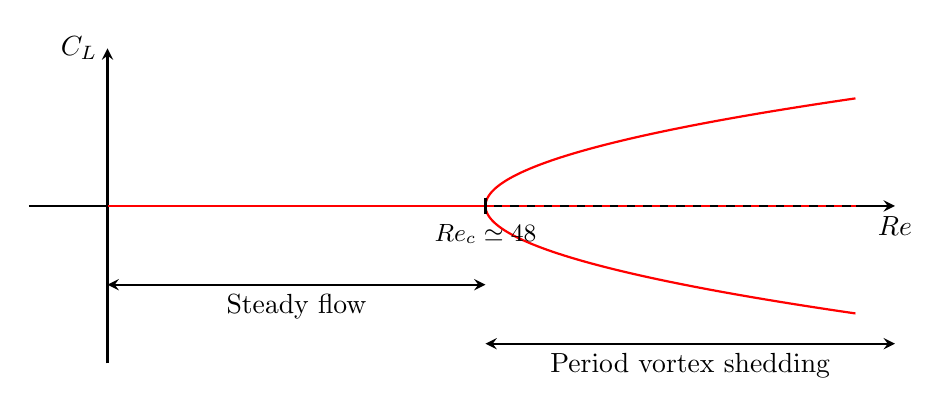
\begin{tikzpicture}[>=stealth]
    \draw[->, thick] (-1, 0) -- (10, 0) node[below] {$Re$};
    \draw[->, thick] (0, -2) -- (0, 2) node[left] {$C_L$};

    \draw[-, thick, red] (0, 0) -- (4.8, 0) node[] {};
    \draw[dashed, thick, red] (4.8, 0) -- (9.5, 0) node[] {};

    \draw[-, thick, red, domain=4.8:9.5, smooth, samples=1024] plot (\x, {0.63*sqrt(\x-4.8}) node[] {};
    \draw[-, thick, red, domain=4.8:9.5, smooth, samples=1024] plot (\x, {-0.63*sqrt(\x-4.8}) node[] {};

    \draw[-, thick] (4.8, 0.1) -- (4.8, -0.1) node[below] {\small $Re_c \simeq 48$};

    \draw[<->, thick] (0, -1) -- (4.8, -1) node[] {};
    \node[below] at (2.4, -1) {Steady flow};

    \draw[<->, thick] (4.8, -1.75) -- (10, -1.75) node[] {};
    \node[below] at (7.4, -1.75) {Period vortex shedding};

  \end{tikzpicture}
\end{frame}





\begin{frame}[t, c]{Two-dimensional cylinder flow}{Finding fixed points}
  \begin{minipage}{.68\textwidth}
    \[
    \tcboxmath[colframe=beamer@kthblue, colback=white]{
      \nabla \cdot \left( \bm{u} \otimes \bm{u} \right) = - \nabla p + \dfrac{1}{Re} \nabla^2 \bm{u}
    }
    \]

    \bigskip

    Define the state vector $\bm{q} = \left( \bm{u}, p \right)^T$.
    Reformulate the problem as a root-finding problem $\mathcal{F}(\bm{q}, Re) = \bm{0}$ and use Newton's method (or variants) to solve it.


  \end{minipage}%
  \hfill
  \begin{minipage}{.28\textwidth}

  \end{minipage}
\end{frame}




\begin{frame}[t, c]{Two-dimensional cylinder flow}{Linear stability analysis}
  \begin{minipage}{.58\textwidth}
    Denote by $\bm{U}_b(\bm{x}, Re)$ the base flow and linearized around it to obtain the linearized system
    %
    \[
    \bm{B} \dfrac{d\bm{q}}{dt} = \bm{Lq}
    \]
    %
    and look for the eigenvalues and eigenvectors of the generalized eigenvalue problem
    %
    \[
    \lambda \bm{B} \hat{\bm{q}} = \bm{L} \hat{\bm{q}}
    \]
    %
    using numerical eigensolvers.
  \end{minipage}%
  \hfill
  \begin{minipage}{.48\textwidth}
  \end{minipage}
\end{frame}




\begin{frame}[t, c]{Two-dimensional cylinder flow}{Linear stability analysis}
  \begin{minipage}{.48\textwidth}
  \end{minipage}%
  \hfill
  \begin{minipage}{.48\textwidth}
  \end{minipage}
\end{frame}




\begin{frame}[t, c]{Two-dimensional cylinder flow}{Linear stability vs.\ real life}
  \centering
  Add evolution of the Strouhal number as a function of Re.
\end{frame}




\begin{frame}[t, c]{Two-dimensional cylinder flow}{Base flow vs.\ mean flow}
  \begin{minipage}{.48\textwidth}
    \centering
    \tcbox[colframe=beamer@kthblue, colback=white]{
      \textbf{Base flow solution}
    }
  \end{minipage}%
  \hfill
  \begin{minipage}{.48\textwidth}
    \centering
    \tcbox[colframe=beamer@kthblue, colback=white]{
      \textbf{Unsteady solution}
    }
  \end{minipage}

  \medskip

  \begin{minipage}{.48\textwidth}
  \end{minipage}%
  \hfill
  \begin{minipage}{.48\textwidth}
  \end{minipage}

\end{frame}





\begin{frame}[t, c]{Two-dimensional cylinder flow}{Base flow vs.\ mean flow}
  \begin{minipage}{.48\textwidth}
    \centering
    \tcbox[colframe=beamer@kthblue, colback=white]{
      \textbf{Base flow solution}
    }
  \end{minipage}%
  \hfill
  \begin{minipage}{.48\textwidth}
    \centering
    \tcbox[colframe=beamer@kthblue, colback=white]{
      \textbf{Time-averaged solution}
    }
  \end{minipage}

  \medskip

  \begin{minipage}{.48\textwidth}
  \end{minipage}%
  \hfill
  \begin{minipage}{.48\textwidth}
  \end{minipage}

\end{frame}





\begin{frame}[t, c]{Two-dimensional cylinder flow}{Modeling objectives}
  \begin{minipage}{.68\textwidth}
    \centering
    \tcbox[colframe=beamer@kthblue, colback=white]{
      \textbf{Objective :} Simple model capturing the essence of the problem.
    }
    
    \bigskip

    \begin{enumerate}
    \item Linearly unstable nature of the fixed point.
    \item Captures the transition to the limit cycle.
    \item Explains why the base flow and mean flow are so different.
    \item Explains why the frequency predictions are bad.
    \item Capture the Reynolds number dependence.
    \end{enumerate}

  \end{minipage}%
  \hfill
  \begin{minipage}{.28\textwidth}
    \centering
    \includegraphics[width=\textwidth]{Gears}
  \end{minipage}

  \vspace{1cm}
\end{frame}





\begin{frame}[t, c]{Two-dimensional cylinder flow}{Modeling strategy}
  \begin{minipage}{.68\textwidth}
    \begin{itemize}
    \item Transform PDE into a handful of ODE.
      %
      \begin{itemize}
      \item[$\hookrightarrow$] Dimensionality reduction, reduced-order modeling, \ldots
      \end{itemize}

      \medskip

    \item Statistical inference of the parameters.
      %
      \begin{itemize}
      \item[$\hookrightarrow$] Least-squares, calibration techniques, interpolation, \ldots
      \end{itemize}

      \medskip

    \item Mathematical analysis of the model's properties.
      %
      \begin{itemize}
      \item[$\hookrightarrow$] Linear and weakly nonlinear analyses, comparison with ground truth, \ldots
      \end{itemize}
    \end{itemize}
  \end{minipage}%
  \hfill
  \begin{minipage}{.28\textwidth}
    \centering
    \includegraphics[width=\textwidth]{Gears}
  \end{minipage}

  \vspace{1cm}
\end{frame}




\begin{frame}[t, c]{Two-dimensional cylinder flow}{Dimensionality reduction}
  \centering
  \includegraphics[width=.8\textwidth]{reduced_order_modeling}
\end{frame}




\begin{frame}[t, c]{Two-dimensional cylinder flow}{Dimensionality reduction}
  \begin{minipage}{.68\textwidth}
    \begin{tcolorbox}[colback=white, colframe=beamer@kthblue]
      \textbf{Objective :} Find proxies for the vortex shedding's amplitude, phase and distortion between the base flow and the mean flow.
    \end{tcolorbox}

    \bigskip

    \begin{itemize}
    \item Snapshots of the full state vector $\left\{ \bm{q}(\bm{x}, t_k) \right\}$ are available :
      \begin{itemize}
      \item[$\hookrightarrow$] use linear dimensionality reduction techniques such as POD/PCA or DMD.
      \end{itemize}

      \medskip

    \item If only limited sensor measurements are available :
      \begin{itemize}
      \item[$\hookrightarrow$] Use time-delay embeddings to construct the proxies.
      \end{itemize}
    \end{itemize}
  \end{minipage}%
  \hfill
  \begin{minipage}{.28\textwidth}
  \end{minipage}
\end{frame}




\begin{frame}[t, c]{Two-dimensional cylinder flow}{Dimensionality reduction}
  \centering
  \includegraphics[width=.8\textwidth]{svd_pod}
\end{frame}




\begin{frame}[t, c]{Two-dimensional cylinder flow}{Dimensionality reduction}
  \begin{minipage}{.68\textwidth}
    \underline{\textbf{Modes 1 and 2 :}} Spatial structure of the vortex shedding.
    Their time-dependant amplitudes provide our proxy variables to describe the evolution of the oscillations.

    \bigskip

    \underline{\textbf{Mode 3 :}} Distortion between the base flow and the mean flow.
    Its amplitude provides the remaining proxy variable for our model.
  \end{minipage}%
  \hfill
  \begin{minipage}{.28\textwidth}

  \end{minipage}

  \vspace{1cm}
\end{frame}




\begin{frame}[t, c]{Two-dimensional cylinder flow}{Low-dimensional representation}
  
\end{frame}




\begin{frame}[t, c]{Two-dimensional cylinder flow}{Low-order model}
  \begin{minipage}{.68\textwidth}
    \begin{tcolorbox}[colframe=beamer@kthblue, colback=white]
      \textbf{Objective :} Obtain a dynamical system describing the evolution of our proxy variables.
    \end{tcolorbox}

    \bigskip

    \begin{itemize}
    \item If the original equations are known :
      \begin{itemize}
      \item[$\hookrightarrow$] Use classical reduced-order modeling techniques (e.g. Galerkin or Petrov-Galerkin projections)
      \end{itemize}

      \medskip

    \item If the original equations are unknown :
      \begin{itemize}
      \item[$\hookrightarrow$] Use data-driven techniques (e.g. system identification or machine learning)
      \end{itemize}
    \end{itemize}
  \end{minipage}%
  \hfill
  \begin{minipage}{.28\textwidth}
    \centering
    \textbf{Model}

    \[
    \dot{\bm{x}} = \bm{f}(\bm{x}, Re)
    \]
  \end{minipage}
\end{frame}





\begin{frame}[t, c]{Two-dimensional cylinder flow}{POD-Galerkin projection}
  \textbf{Step 1 :} Galerkin expansion of the velocity field as
  %
  \[
  \bm{u}(\bm{x}, t) \simeq \bm{U}_b(\bm{x}) + \bm{u}_1(\bm{x}) a_1(t) + \bm{u}_2(\bm{x}) a_2(t) + \bm{u}_{\Delta} a_{\Delta}(t) + \cdots
  \]

  \medskip

  \textbf{Step 2 :} Inject the Galerkin expansion into the Navier-Stokes equations and project onto the span of the POD modes.
  %
  \[
  \bm{U}^T \bm{U} \dfrac{d \bm{a}}{dt} = \bm{U}^T \bm{f}(\bm{Ua}, Re)
  \]

  \medskip

  \textbf{Step 3 :} Inspect the model and use for rapid (approximate) simulations of the original system.
\end{frame}




\begin{frame}[t, c]{Two-dimensional cylinder flow}{POD-Galerkin reduced-order model}
  \centering
  \begin{tcolorbox}[colback=white, colframe=beamer@kthblue]
    \centering
    \textbf{Reduced-order model}
    %
    \[
    \begin{aligned}
      \dot{x} & = \sigma x - \omega y - xz - \alpha yz \\
      \dot{y} & = \omega x + \sigma y - yz + \alpha xz \\
      \dot{z} & = -z + x^2 + y^2
    \end{aligned}
    \]
  \end{tcolorbox}
\end{frame}




\begin{frame}[t, c]{Two-dimensional cylinder flow}{POD-Galerkin reduced-order model}
  
\end{frame}




\begin{frame}[t, c]{Two-dimensional cylinder flow}{Physical analysis}
  \begin{minipage}{.68\textwidth}
    \begin{tcolorbox}[colback=white, colframe=beamer@kthblue]
      \textbf{Objective :} What can this model tell us about the physics of the problem and to what extent is it correct?
    \end{tcolorbox}

    \bigskip

    \begin{itemize}
    \item \textbf{Physical consistency :}
      \begin{itemize}
      \item[$\hookrightarrow$] Does it respect the known physics?
      \item[$\hookrightarrow$] Are its predictions consistent with the observations?
      \end{itemize}

      \medskip

    \item \textbf{Improved understanding :}
      \begin{itemize}
      \item[$\hookrightarrow$] What does it tells us about the problem which was not directly obvious?

      \item[$\hookrightarrow$] What insights are to be gained?
      \end{itemize}
    \end{itemize}
  \end{minipage}%
  \hfill
  \begin{minipage}{.28\textwidth}
    \centering
    \includegraphics[width=\textwidth]{Gears}
  \end{minipage}
\end{frame}




\begin{frame}[t, c]{Two-dimensional cylinder flow}{Reduced-order model consistency}
  \begin{tcolorbox}[colback=white, colframe=beamer@kthblue]
    \textbf{Property :} The quadratic nonlinear term in Navier-Stokes equations is energy-preserving.
  \end{tcolorbox}
  
  \bigskip
  
  The kinetic energy is given by $E(t) = \| \bm{a}(t) \|_2^2$ and we thus have
  %
  \[
  \begin{aligned}
    \dfrac{dE}{dt} & = \dfrac{1}{2} \bm{a}^T \dot{\bm{a}} \\
    & = \dfrac{1}{2} \left( x  \dot{x} + y \dot{y} + z \dot{z} \right) \\
    & = \sigma (x^2 + y^2) - z^2
  \end{aligned}
  \]
  %
  Only the linear terms in our model contribute to this energy budget.
\end{frame}




\begin{frame}[t, c]{Two-dimensional cylinder flow}{Reduced-order model consistency}
  \begin{tcolorbox}[colback=white, colframe=beamer@kthblue]
    \textbf{Property :} The fixed point has a two-dimensional unstable subspace characterized by complex-conjugate eigenvalues.
  \end{tcolorbox}
  
  \bigskip
  
  The Jacobian matrix of the system reads
  %
  \[
  \bm{J} = \begin{bmatrix}
    \sigma - z & -\omega - \alpha z & -x - \alpha y \\
    \omega + \alpha z & \sigma - z & -y + \alpha x\\
    2x & 2y & -1
  \end{bmatrix}
  \]
  %
  For $(x, y, z) = (0, 0, 0)$ and $\sigma > 0$, its eigenvalues are $\sigma \pm i \omega$ and $-1$.
\end{frame}




%% \begin{frame}[t, c]{Two-dimensional cylinder flow}{Reduced-order model consistency}
  
%% \end{frame}




\begin{frame}[t, c]{Two-dimensional cylinder flow}{What insights are to be gained?}
  \begin{minipage}{.68\textwidth}
    \centering
    What can this reduced-order model actually tell me about the two-dimensional cylinder flow ?
  \end{minipage}%
  \hfill
  \begin{minipage}{.28\textwidth}
    \[
    \begin{aligned}
      \dot{x} & = \sigma x - \omega y - xz - \alpha yz\\
      \dot{y} & = \omega x + \sigma y - yz + \alpha xz \\
      \dot{z} & = -z + x^2 + y^2
    \end{aligned}
    \]
  \end{minipage}
\end{frame}





\begin{frame}[t, c]{Two-dimensional cylinder flow}{What insights are to be gained?}
  \begin{overprint}
    \onslide<1>
    \[
    \begin{aligned}
      \dot{x} & = \sigma x - \omega y - xz - \alpha yz\\
      \dot{y} & = \omega x + \sigma y - yz + \alpha xz \\
      \dot{z} & = -z + x^2 + y^2
    \end{aligned}
    \]
    
    \onslide<2>
    \[
    \begin{aligned}
      \dot{\eta} & = \left( \sigma + i \omega \right) \eta - \eta z + i \alpha z \\
      \dot{z} & = - z + \vert \eta \vert^2
    \end{aligned}
    \]
    
    \onslide<3>
    \[
    \begin{aligned}
      \dot{r} & = \left( \sigma - z \right) r\\
      \dot{\varphi} & = \omega + \alpha z\\
      \dot{z} & = -z + r^2
    \end{aligned}
    \]
    
  \end{overprint}
\end{frame}

\begin{frame}[t, c]{Two-dimensional cylinder flow}{What insights are to be gained?}
  \begin{minipage}{.68\textwidth}
    Both the linearly unstable \alert{\textbf{baseflow}} \( (r, z) = (0, 0) \) and linearly stable \alert{\textbf{mean flow}} \( (r, z) = (\bar{r}, \bar{z}) \) are fixed points of the \alert{\textbf{phase-averaged}} equations.

    \bigskip

    Given that $\dot{\varphi} = \omega + \alpha z$, the instantaneous frequency of the vortex shedding changes as the flow is distorted from the baseflow to the mean flow.
  \end{minipage}%
  \hfill
  \begin{minipage}{.28\textwidth}

  \end{minipage}
\end{frame}





\begin{frame}[t, c]{Two-dimensional cylinder flow}{What insights are to be gained?}
  \begin{minipage}{.48\textwidth}
    \[
    \textbf{Distortion eq :} \quad \dot{z} = -z + r^2
    \]
  \end{minipage}%
  \hfill
  \begin{minipage}{.48\textwidth}
    \[
    \textbf{Amplitude eq :} \quad \dot{r} = \left( \sigma - z \right) r
    \]
  \end{minipage}

  \bigskip

  \begin{minipage}{.48\textwidth}
    As $r$ increases, the amplitude $z$ of the distortion increases.
    It does so until a balance is met where $z = r^2$.
    Here, $r^2$ plays the role of the \alert{\textbf{Reynolds stesses}} in the Navier-Stokes eqn.
  \end{minipage}%
  \hfill
  \begin{minipage}{.48\textwidth}
    $\sigma - z$ is the \alert{\textbf{effective growth rate}} of the instability.
    The amplitude of the vortex shedding grows until a balance is met where $z = \sigma$.
    \vspace{0.5cm}
  \end{minipage}

\end{frame}




\begin{frame}[t, c]{Two-dimensional cylinder flow}{What insights are to be gained?}
  
\end{frame}



\begin{frame}[t, c]{Two-dimensional cylinder flow}{Two-timing approximate solution}
  Assume that $\sigma = \epsilon^2$ and introduce a multiple time-scale expansion with $\tau = \epsilon^2 t$.
  Expanding the solution in the vicinity of $(r_0, z_0) = (0, 0)$ yields
  %
  \[
  \begin{aligned}
    r(t, \epsilon) & = \epsilon r_1(t, \tau) + \epsilon^2 r_2(t, \tau) + \epsilon^3 r_3(t, \tau) + \cdots \\
    z(t, \epsilon) & = \epsilon z_1(t, \tau) + \epsilon^2 z_2(t, \tau) + \epsilon^3 z_3(t, \tau) + \cdots
  \end{aligned}
  \]
  %
  We can now use \alert{\textbf{regular perturbation theory}} to obtain an approximation of the evolution of $r(t)$ and $z(t)$.
\end{frame}




\begin{frame}[t, c]{Two-dimensional cylinder flow}{Two-timing approximate solution}
  \begin{minipage}{.68\textwidth}
    After some algebraic manipulations, we obtain that the vortex shedding's amplitude obeys
    %
    \[
    \dfrac{dr}{dt} = \sigma  r - r^3
    \]
    %
    while the evolution of the distortion is given by
    %
    \[
    z(t) = A e^{-t} + r^2(t) \left(1 - e^{-t}\right) + \mathcal{O}(\epsilon^3).
    \]
    %
    and so, very rapidly we have $z(t) \approx r^2(t)$.
  \end{minipage}%
  \hfill
  \begin{minipage}{.28\textwidth}
  \end{minipage}
\end{frame}




\begin{frame}[t, c]{Two-dimensional cylinder flow}{Further reducing the model's complexity\ldots}
  \begin{minipage}{.48\textwidth}
    \[
    \begin{aligned}
      \dot{r} & = \sigma r - r^3 \\
    \dot{\varphi} & = \omega + \alpha z \\
    z & = r^2
    \end{aligned}
    \]
  \end{minipage}%
  \hfill
  \begin{minipage}{.48\textwidth}

  \end{minipage}
\end{frame}




\begin{frame}[t, c]{Two-dimensional cylinder flow}{Piecing everything together}

\end{frame}




\begin{frame}[t, c]{Two-dimensional cylinder flow}{The power of mathematical modeling}
  \begin{minipage}{.68\textwidth}
    Our model explains most of the dynamics observed in the flow :

    \medskip

    \begin{itemize}
    \item Saturation mechanism for the vortex shedding's amplitude,
    \item The baseflow gets distorted into the mean flow through the Reynold stresses,
    \item This distortion simultaneously induces a frequency shift.
    \end{itemize}

    \medskip

    To date, this is the simplest yet most accurate reduced-order model of the cylinder flow.
  \end{minipage}%
  \hfill
  \begin{minipage}{.28\textwidth}
  \end{minipage}
\end{frame}




\begin{frame}[t, c]{Two-dimensional cylinder flow}{What next ?}
  \begin{minipage}{.68\textwidth}
    Despite its accuracy and interpretability, our model leaves some questions unanswered, e.g.

    \medskip

    \begin{itemize}
    \item What is the physical mechanism responsible for the instability in the first place ?
    \item How exactly does the spatial support of the different structures evolves as their amplitude grows ?
    \item To what extent is our model generic and applicable to other flows ?
    \end{itemize}

    \medskip

    This is where we leave the realm of dynamical systems and enter that of classical fluid mechanics.

  \end{minipage}%
  \hfill
  \begin{minipage}{.28\textwidth}
  \end{minipage}
\end{frame}

\begin{frame}
\end{frame}


\end{document}
